\documentclass[a4paper, 11pt]{article}

\usepackage[utf8x]{inputenc}
\usepackage[portuguese]{babel}
\usepackage[pdfborder={0 0 0}]{hyperref}
\usepackage{graphicx}
\usepackage{float}
\usepackage{amsmath, amssymb, amsfonts, amsthm}
\usepackage{a4wide}
\usepackage{indentfirst}
\usepackage{multicol}
\usepackage[cache=false]{minted}
\usepackage{subcaption}
\usepackage{fancyhdr}
\usepackage{lastpage}
\usepackage{relsize}
\usepackage[justification=centering]{caption}

\title{Computação Gráfica \\ [0.8em] \smaller{} Fase IV -- Normais e Coordenadas de Textura}
\author{João Neves (a81366) \and Luís Manuel Pereira (a77667) \and Rui Fernandes (a89138)
\and Tiago Ribeiro (a76420)}
\date{Maio 2021}

\renewcommand\labelitemi{--}

\begin{document}

\begin{titlepage}
    \begin{center}
        \begin{minipage}{.75\linewidth}
            \centering
            
\includegraphics[width=0.4\textwidth]{img/EEUM.png}\par\vspace{1cm}
            \vspace{1.5cm}
            \href{https://www.uminho.pt/PT}{\scshape\LARGE Universidade do Minho} \par
            \vspace{1cm}
            \href{https://www.di.uminho.pt/}{\scshape\Large Departamento de Informática} \par
            \vspace{1.5cm}
            \maketitle
        \end{minipage}
    \end{center}
    \vspace{2cm}
    \thispagestyle{empty}
    \clearpage
\end{titlepage}

\pagenumbering{roman}

\begin{abstract}
O presente relatório descreve o trabalho prático realizado no âmbito da disciplina de 
\href{https://miei.di.uminho.pt/plano_estudos.html#computa_o_gr_fica}{\emph{Computação 
Gráfica}}, ao longo do segundo semestre
do terceiro ano do \href{http://miei.di.uminho.pt}{Mestrado Integrado em Engenharia Informática} 
da \href{https://www.uminho.pt}{Universidade do Minho}.

Esta fase consiste na adição de novas funcionalidades e modificações ao trabalho já realizado, 
tais como o uso de texturas e a aplicação de iluminação, por forma a obter representações 
mais realistas dos sistemas a representar.

Neste documento descrevemos sucintamente a aplicação desenvolvida discutimos as decisões tomadas 
durante a realização do trabalho prático.
\end{abstract}

\pagebreak

\tableofcontents
\listoffigures

\pagebreak

\pagenumbering{arabic}

\pagestyle{fancy}
\fancyhf{}

\rfoot{Página \thepage \hspace{1pt} de \pageref{LastPage}}

\renewcommand{\headrulewidth}{0pt}

\section{Introdução}

Nesta quarta e última fase do projeto proposto no âmbito da unidade curricular de Computação 
Gráfica, damos seguimento ao trabalho desenvolvido nas fases anteriores. Nesta fase pretende-se 
estender a aplicação de modo a que o gerador de primitivas gere, para além das coordenadas de 
cada vértice, as normais e coordenadas de textura.

Relativamente ao motor gráfico, este deve ser suportar as funcionalidades de iluminação e 
texturização, assim como possibilitar a pormenorização de cores e texturas no ficheiro XML.

Dito isto, nos capítulos que se seguem será explicado, detalhadamente, todo o processo para obter 
os resultados pretendidos.

\pagebreak

\section{\textit{Generator}}

Até à fase anterior, o \textit{generator} gerava as coordenadas dos pontos constituintes de cada  
um dos modelos. No entanto, de forma a poder prosseguir à aplicação de texturas, este deve ser 
alterado de modo a calcular também as coordenadas normais e de textura de cada um dos ponto.

\subsection{Ficheiros XML}

De maneira a ser possível implementar as novas funcionalidades, foi necessária a adição de 
novas \textit{tags} e atributos ao ficheiro XML da fase anterior.

Uma vez que todos os elementos da cena passam a possuir textura, foi adicionado dentro de cada 
modelo, junto ao atributo \textit{file} que indica o ficheiro \texttt{.3d} utilizado, o atributo 
\textit{texture} que referencia imagem representativa da textura.

\begin{minted}{xml}
<models>
    <model file="sphere.3d" texture="../textures/2k_jupiter.jpg" /> 
</models>
\end{minted}

Para além disso, foi também adicionada a indicação de todas as luzes a ser consideradas: 

\begin{minted}{xml}
<lights>
    <light type="POINT" posX="0" posY="0" posZ="0" diffR="1" diffG="1"
           diffB="1" />
</lights>
\end{minted}

Por fim, adicionou-se, também, as características dos materiais associados a cada uma das 
primitvas:

\begin{minted}{xml}
<models>
    <model file="sphere.3d" diffR="0.1" diffG="0.2" diffB="0.3" />
</models>
\end{minted}

Tendo estes aspetos em consideração, é possível notar que o ficheiro XML evoluiu bastante ao 
longo das fases, passando de um simples ficheiro com primitivas geométricas, a um ficheiro 
complexo onde existem transformações geométricas, curvas, texturas e luzes. 

\subsection{Normais \& Coordenadas de Textura}

As normais de cada um dos vértices são gerados para que, a partir de uma fonte de luz, seja 
possível gerar uma sombra. 

De modo a obter as normais para os diferentes vértices de cada figura, foi necessário efetuar um 
estudo de cada triângulo que constitui a mesma. É, assim, necessário obter um vetor normal para 
cada vértice, \textit{i.e.} um vetor perpendicular à superfície nesse ponto.

Por outro lado, para conseguir inserir texturas nos objetos, surge a necessidade de definir os 
pontos textura para cada uma das figuras.

Desta forma, é necessário o estudo de um plano 2D para a figuras geométricas tridimensionais, 
usando como revestimento das mesmas. O mapeamento é feito da seguinte forma:

\begin{figure}[H]
	\centering
	\begin{subfigure}{.35\textwidth}
		\centering
		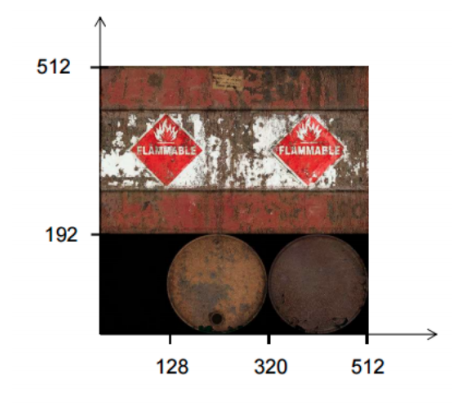
\includegraphics[width=\textwidth]{img/text1.png}
		\caption{Espaço da imagem real}
	\end{subfigure}%
	\begin{subfigure}{.35\textwidth}
		\centering
		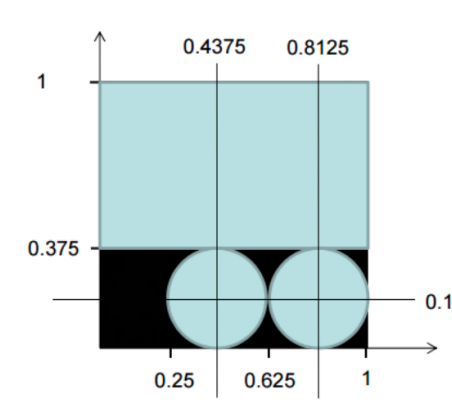
\includegraphics[width=\textwidth]{img/text2.png}
		\caption{Espaço da textura}
	\end{subfigure}
	\caption{Mapeamento de texturas}
\end{figure}

Tal como se pode verificar na figura anterior, estabelece-se que o eixo cartesiano da textura tem 
como limite máximo 1 e um limite mínimo de zero. Importa notar que estes limites correspondem aos 
limites da imagem real, no entanto, mapeados para valores no intervalo $\left[ 0, 1 \right]$, 
usando o canto inferior esquerdo de todas as imagens como origem.

\subsubsection{Plano}

Tendo em conta a orientação do plano, isto é, se este se encontra de frente para o ecrã ou 
virado na mesma direção (ordem dos pontos), as normais serão um vetor constituído pela 
orientação e valores nulos nos restantes eixos. 

Por exemplo, para um plano no eixo $xOz$, com $y = 0$ as normais dos pontos serão $(0, 1, 0)$, tal 
como representado na Figura \ref{fig:plane}.

\begin{figure}[H]
    \centering
    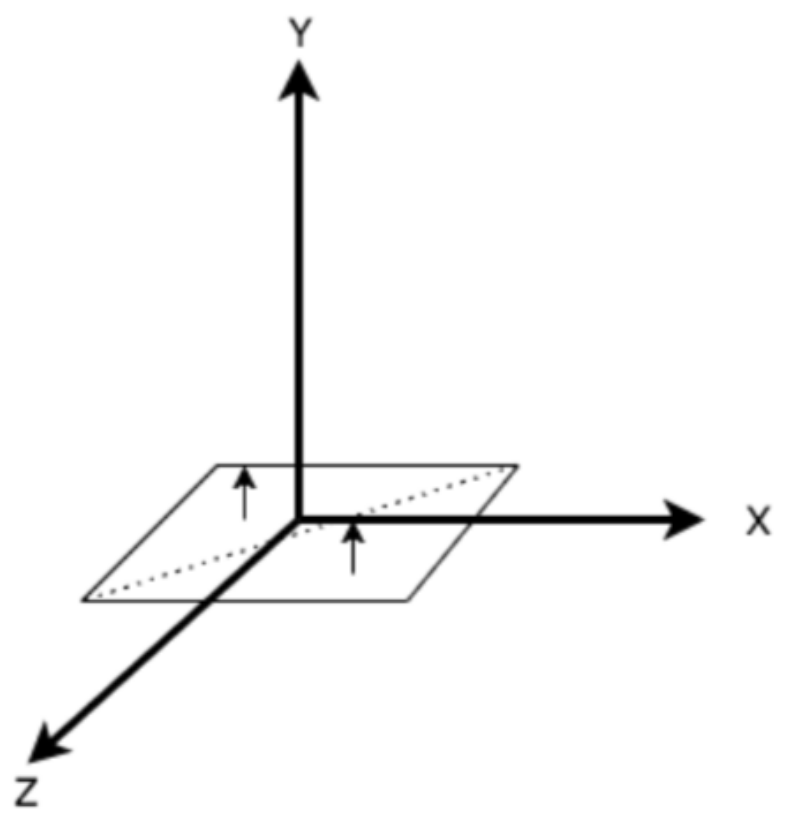
\includegraphics[width=.3\textwidth]{img/xoz.png}
    \caption{Vetores normais ao plano $xOz$}
    \label{fig:plane}
\end{figure}

O processo de obtenção das coordenadas de textura é simples no caso desta figura geométrica. O 
formato é o mesmo que o da imagem 2D, sendo apenas necessário fazer a correspondência direta de 
cada vértice do plano com os vértices da imagem 2D, tal como ilustrado de seguida.

\begin{figure}[H]
    \centering
    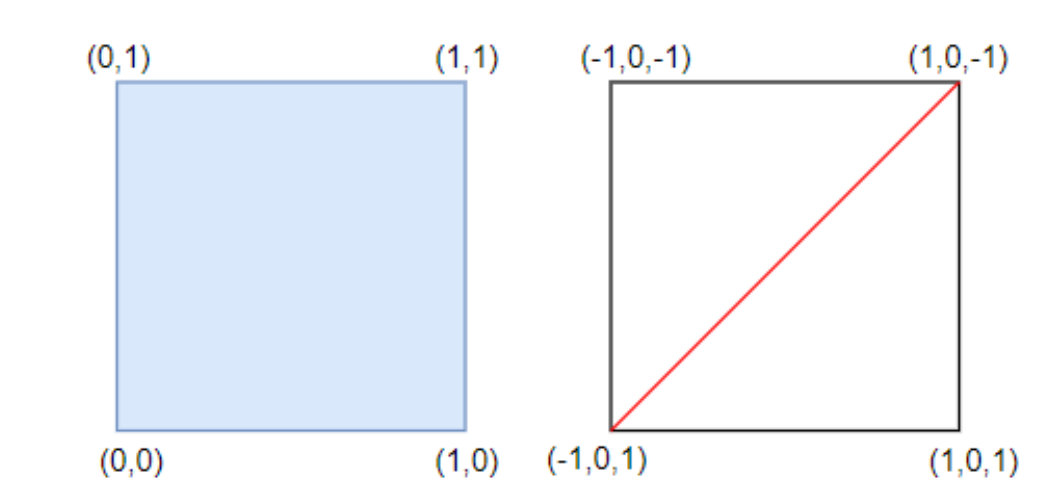
\includegraphics[width=.5\textwidth]{img/text_plane.png}
    \caption{Coordenadas das texturas (à esquerda) e coordenadas dos vértices do plano (à 
direita)}
\end{figure}

\subsubsection{Paralelepípedo}

Seguindo um raciocínio análogo, o cálculo dos vetores normais associados a um paralelepípedo 
torna-se trivial. Desta forma, tal como ilustrado na Figura \ref{fig:box}, dependendo da face em 
questão, os vetores normais serão os seguintes:

\begin{multicols}{2}
\begin{itemize}
    \item Face Frontal: $(0, 0, 1)$
    \item Face Traseira: $(0, 0, -1)$
    \item Face Direita: $(1, 0, 0)$
    \item Face Esquerda: $(-1, 0, 0)$
    \item Topo: $(0, 1, 0)$
    \item Base: $(0, -1, 0)$
\end{itemize}
\end{multicols}

\begin{figure}[H]
    \centering
    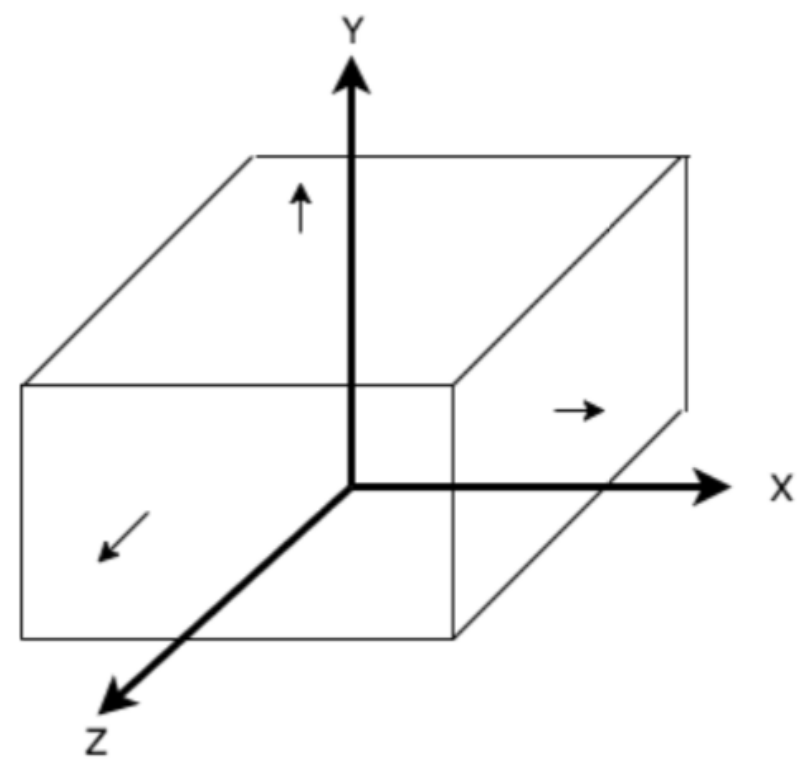
\includegraphics[width=.3\textwidth]{img/box.png}
    \caption{Vetores normais ao paralelepípedo}
    \label{fig:box}
\end{figure}

\pagebreak

Para a obtenção das coordenadas de textura do paralelepípedo, estabeleceu-se uma imagem 2D como 
regra possuindo sempre o seguinte formato:

\begin{figure}[H]
    \centering
    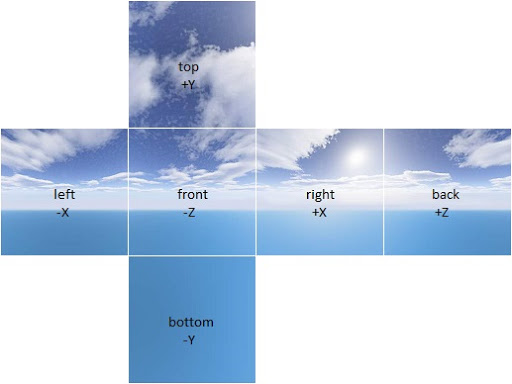
\includegraphics[width=.6\textwidth]{img/cubemap.jpg}
    \caption{Formato da textura de um paralelepípedo}
\end{figure}

Desta forma, para calcular as coordenadas de textura, obtém-se a posição da imagem a que 
corresponde a face em questão e itera-se no mesmo sentido e, que o paralelepípedo é desenhado, 
atribuindo textura a cada vértice o ponto de textura correspondente.

\subsubsection{Cone}

O cone possui dois tipos de normais, as da sua base e as da sua superfície lateral. Sendo assim, 
as normais referentes à base do cone são dadas pelo vetor $(0, −1, 0)$.

No que diz respeito à superfície do cone, a determinação dos vetores normais é realizada em  
dois passos. Primeiro, determinam-se os vetores normais para uma circunferência paralela à base, 
como a representada em seguida:

\begin{figure}[H]
    \centering
    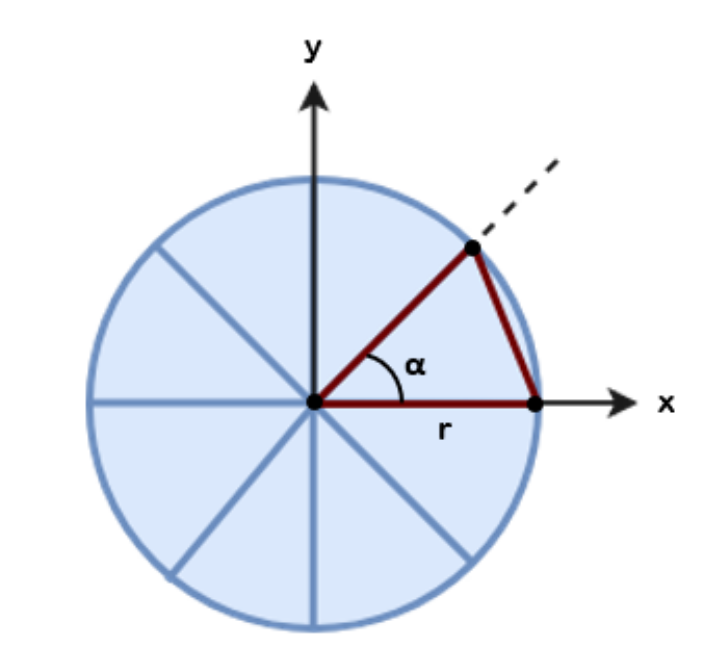
\includegraphics[width=.4\textwidth]{img/esfera_normal.png}
    \caption{Circunferência paralela à base de um cone}
\end{figure}

De seguida, representando por $h$ a altura do cone e por $r$ o raio da base, determina-se a 
inclinação do clone, $\theta$, da seguinte forma: $$\tan(\theta) = \frac{h}{r} \Leftrightarrow 
\theta = \arctan \left( \frac{r}{h} \right)$$

Por fim, tal como ilustrado na Figura \ref{fig:cone}, um vértice na superfície lateral do cone 
terá como vetor normal o seginte vetor: $$\overrightarrow{N} = (\cos(\alpha) \times \cos(\theta), 
\ \sin(\theta), \ \sin(\alpha) \times \cos(\theta))$$

 
\begin{figure}[H]
    \centering
    
\includegraphics[width=.5\textwidth]{img/cone.png}
    \caption{Vetores normais ao cone}
    \label{fig:cone}
\end{figure}

De forma a aplicar texturas, começou-se por definir o formato que estas terão, representado em 
seguida:

\begin{figure}[H]
    \centering
    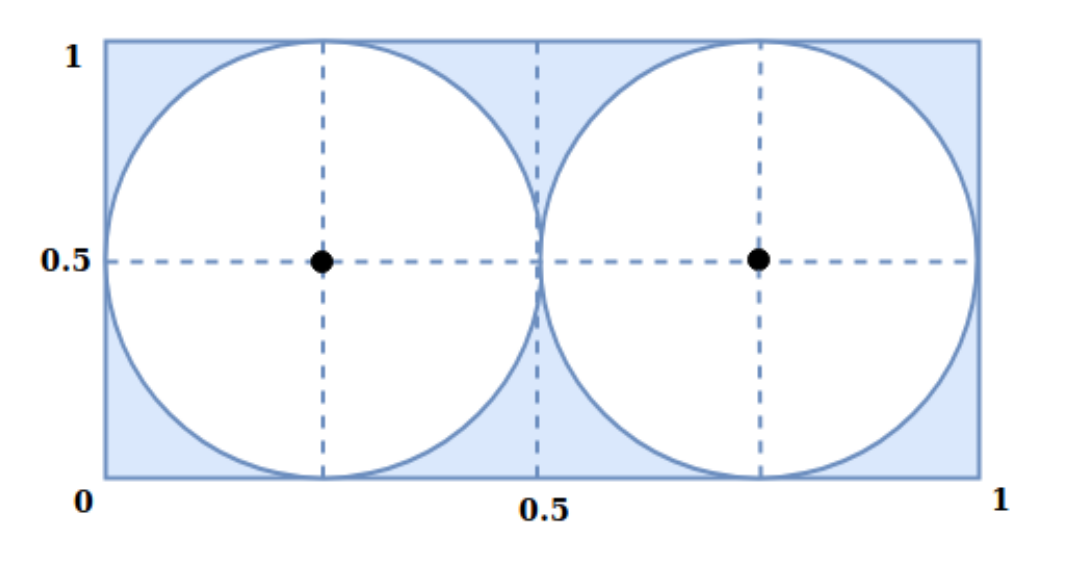
\includegraphics[width=.5\textwidth]{img/text_cone.png}
    \caption{Formato da textura de um cone}
\end{figure}

Deste modo, definiu-se a circunferência da esquerda como sendo a representação da base do cone, 
enquanto a da direita representa a sua superfície lateral lateral.

\pagebreak

\subsubsection{Esfera}

O cálculo dos vetores normais à esfera é realizado tendo em conta a origem da mesma e um ponto 
arbitrário que esteja presente nela. Uma vez que a própria representação da esfera já se 
baseia neste pressuposto, conclui-se que o valor das normais da figura poderá corresponder às 
coordenadas destes pontos. Ou seja, o vetor das normais poderá ser representado como 
$\overrightarrow{N} = \overrightarrow{OP} = P - O = P$.

\begin{figure}[H]
    \centering
    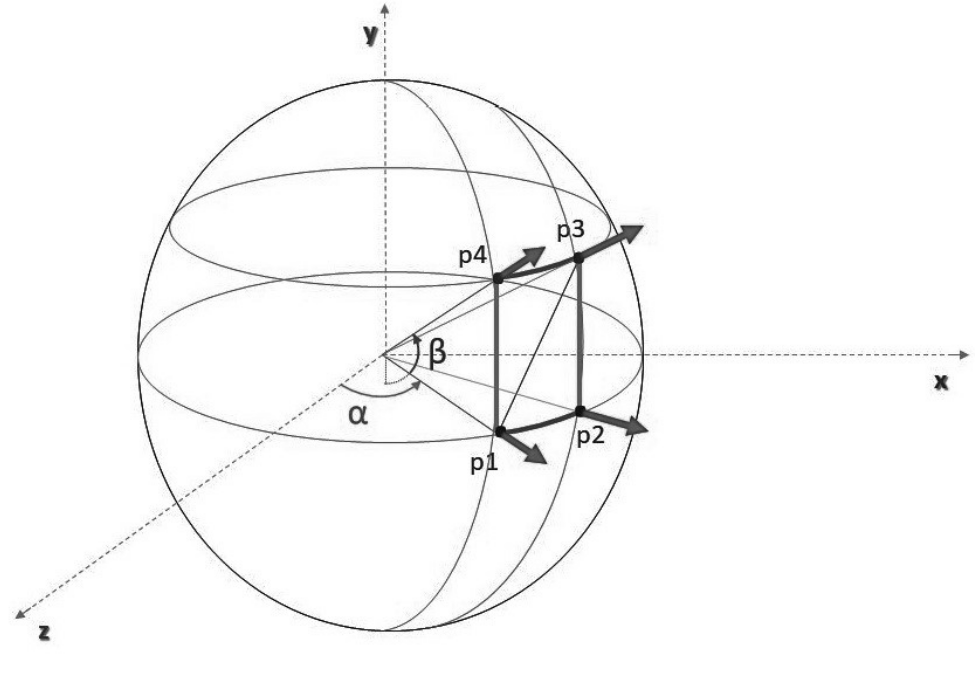
\includegraphics[width=.5\textwidth]{img/esfera.png}
    \caption{Vetores normais à esfera}
\end{figure}

Para associar um vértice a um ponto de textura, apenas é necessário conhecer o número de 
\textit{stacks} e \textit{slices}. Assim, conhecendo o valor da variação associada a cada um 
destes parâmetros e a ordem dos pontos na criação da esfera, é possível mapear facilmente a 
textura.

Assim, para cada vértice $(i, j)$, a sua textura será: 

$$\left(\frac{j}{slices} , \frac{i}{stacks}\right)$$

\subsubsection{\textit{Torus}}

Por forma a obter os vetores normais ao \textit{torus}, aplicou-se o mesmo raciocínio que 
utilizado na esfera, em que o próprio ponto corresponde à sua normalização. Desta forma, as 
expressões ficam iguais às da esfera.

\begin{figure}[H]
    \centering
    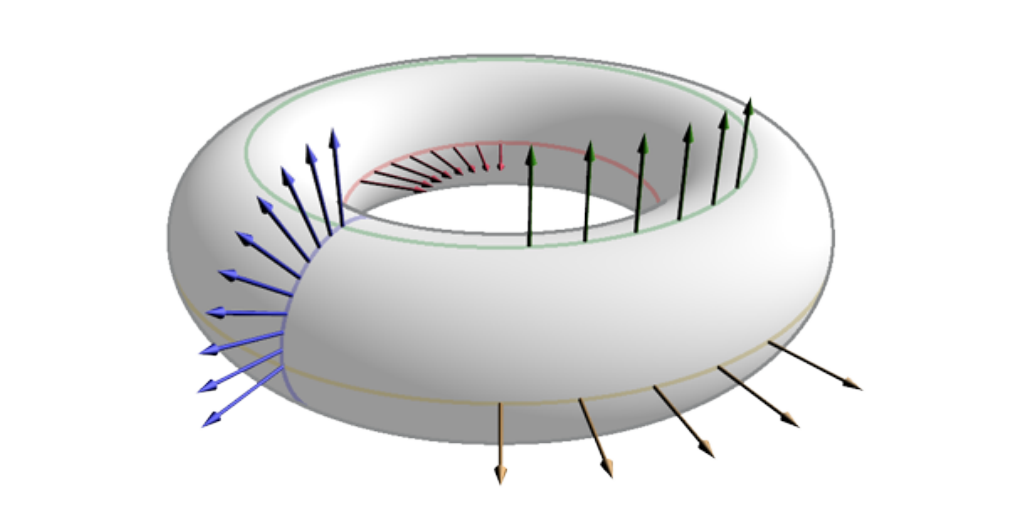
\includegraphics[width=.4\textwidth]{img/torus.png}
    \caption{Vetores normais ao \textit{torus}}
\end{figure}

Quanto às coordenadas das texturas, cada anel do \textit{torus} corresponde a uma textura, fazendo 
com que chegando ao fim de todas as iterações tenha sido preenchido cada um destes anéis, 
estando, portanto, o \textit{torus} preenchido na totalidade.

\subsubsection{\textit{Patches} de Bézier}

Para calcular as normais de um dado ponto $(u, v)$ de uma superfície de Bezier, recorre-se às 
seguintes equações:

\begin{equation*}
    \frac{\partial B(u, v)}{\partial u} = 
    \begin{bmatrix} 3u^2 & 2u & 1 & 0  \end{bmatrix} 
    M 
    P M^T V^T
\end{equation*}

\begin{equation*}
\frac{\partial B(u, v)}{\partial u} = UM
    P  
	M^T
	\begin{bmatrix}
	    3v^2 \\ 2v \\ 1 \\ 0 \\ 
	\end{bmatrix}
\end{equation*}

\

Tendo as derivadas parciais, o vetor normal a qualquer ponto na superfície é o resultado 
normalizado do produto externo dos vetores tangentes ao ponto (sendo eles o resultado das duas 
equações acima). Relativamente às texturas, a um ponto $(u,v)$ corresponde a textura $(u, v)$, 
uma vez que $u$ e $v$ variam no intervalo $\left[ 0, 1 \right]$, tal como a textura.

\pagebreak

\section{\textit{Engine}}

O \textit{engine} é responsável pelo armazenamento da informação dos modelos a representar, 
assim como as respetivas transformações geométricas de cada um desses modelos, que no seu 
conjunto, irão formar o modelo do Sistema Solar que se pretende representar. 

Esta aplicação também sofreu alterações na sua implementação, resultantes da necessidade de 
incorporar novas características dos modelos -- \textit{iluminação}. Findando o processo de 
leitura do ficheiro, passamos para a fase seguinte, a qual é responsável pela renderização da 
informação previamente obtida.

\subsection{Iluminação}

A iluminação dos modelos gerados no projeto é corretamente obtida através do cálculo das 
várias normais, sendo que é através destas que se determina a intensidade da luz.

\subsubsection*{Posição}

Para a criação de diferentes cenários e de modo a permitir uma simulação mais realista foram 
usados tipos diferentes de luz:

\begin{itemize}
    \item \texttt{POINT} -- Trata-se de uma luz que é posicionada num ponto e emite feixes de luz 
em todas as direções à sua volta;
    \item \texttt{DIRECTIONAL} -- Trata-se de uma luz que vem de um ponto no infinito e tem uma 
direção apenas de maneira a atingir o cenário de uma só direção.
\end{itemize}

\subsubsection*{Cor}

De forma a ser possível ter uma perceção complexa e real da luz e da sua reflexão por parte dos 
objetos, a cor deve possuir um total de 4 parâmetros:

\begin{itemize}
    \item \texttt{GL\_AMBIENT} -- Corresponde à cor de um objeto quando este se encontra à 
sombra, ou seja, não existe nenhum feixe de luz que o atija;
    \item \texttt{GL\_DIFFUSE} -- Este componente representa a cor do objeto, \textit{i.e.}, a cor 
que possui quando atingido com uma luz branca;
    \item \texttt{GL\_EMISSION} -- Cor da luz emitida por um objeto;
    \item \texttt{GL\_SPECULAR} -- Cor da reflexão especular característica a uma superfície 
brilhante.
\end{itemize}

\pagebreak

Na Figura \ref{fig:phong}, encontra-se um representado um exemplo de como alguns dos diferentes 
parâmetros mencionados afetam  a visualização do objeto.

\begin{figure}[H]
    \centering
    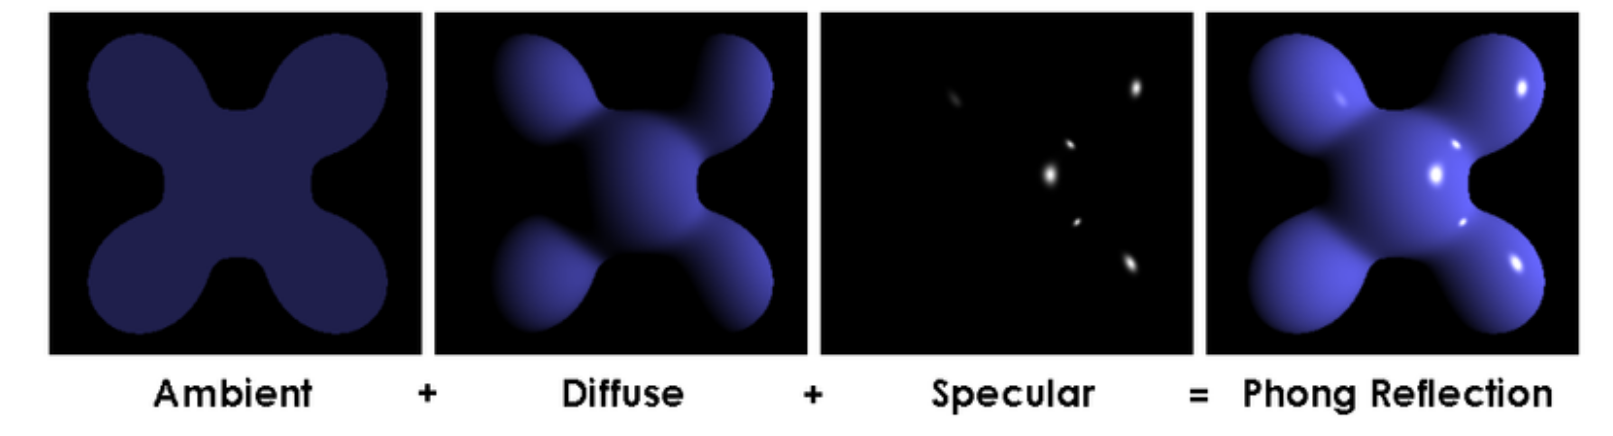
\includegraphics[width=\textwidth]{img/phong.png}
    \caption{Modelo de Iluminação de Phong}
    \label{fig:phong}
\end{figure}

Tendo em conta os aspetos supramencionados, apresentam-se, de seguida, alguns exemplos da 
aplicação de texturas e iluminação:

\begin{figure}[H]
	\centering
	\begin{subfigure}{.5\textwidth}
		\centering
		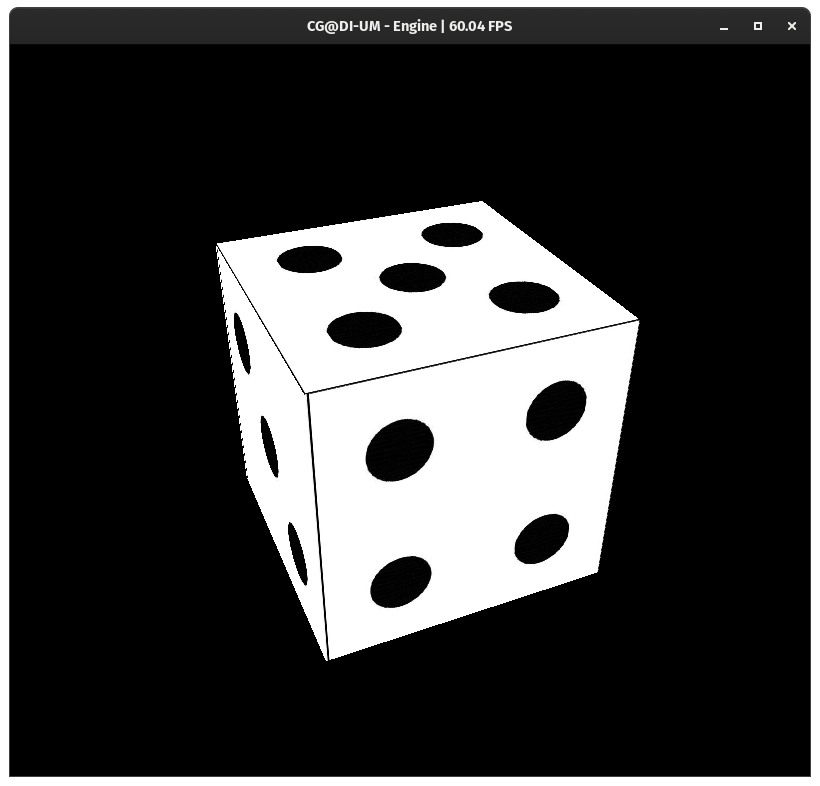
\includegraphics[width=\textwidth]{img/dart.png}
		\caption{Textura aplicada a um paralelepípedo}
	\end{subfigure}%
	\begin{subfigure}{.5\textwidth}
		\centering
		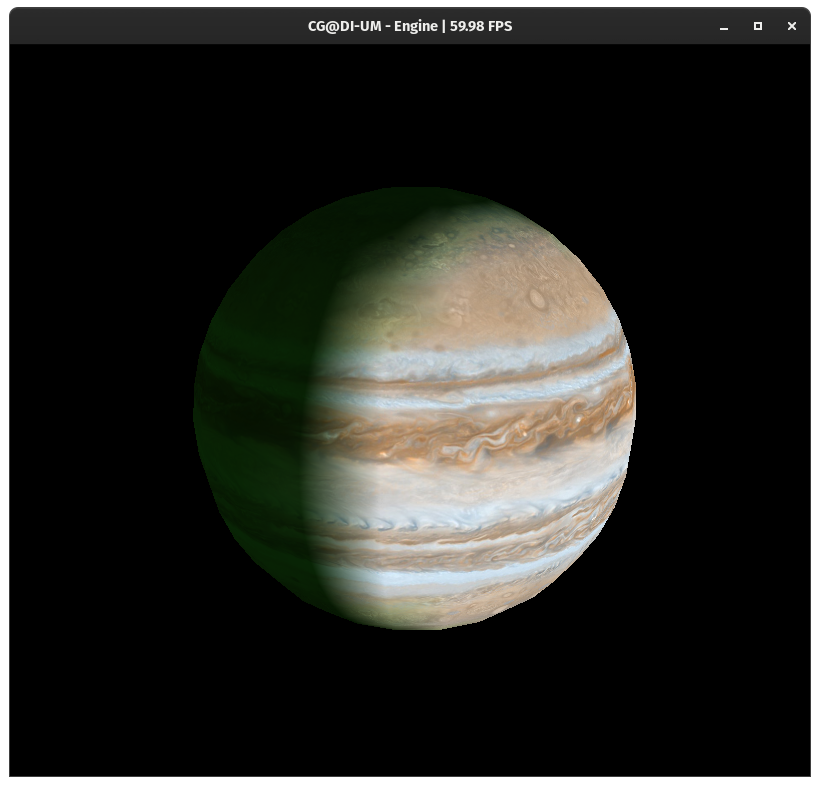
\includegraphics[width=\textwidth]{img/esfera1.png}
		\caption{Textura e iluminação aplicada a uma esfera}
	\end{subfigure}
	\caption{Aplicação de Texturas e Iluminação}
\end{figure}

\subsection{\textit{VBOs}}

Tal como na fase anterior continuamos a fazer uso de VBOs (\textit{Vertex Buffer Object}) para 
passar diretamente para a placa gráfica um \textit{array} com as coordenadas dos vértices dos 
objetos a serem gerados. Com a implementação de texturas e iluminação, tornou-se, então, 
necessário criar  mais 2 \textit{VBOs}, um com as normais e outra com a textura de cada um dos 
pontos.


\pagebreak

\section{Análise de Resultados}

O resultado final do modelo Sistema Solar desenvolvido ao longo do projeto correspondeu às 
expectativas do grupo. Todos os planetas foram representados a uma escala próxima da real, sendo 
sujeitas a ligeiros ajustes para permitir uma maior clareza, os seus tempos de rotação e 
translação têm em  consideração as diferenças reais entre corpos celestes, e alguns 
satélites naturais foram representados, de modo a tornar o cenário o mais agradável possível.

Por fim, importa salientar que, para além do apresentado nestas imagens, o \textit{engine} é 
capaz de processar qualquer uma das primitivas geométricas definidas nas fases anteriores, 
aplicando-lhes texturas e iluminação.

Apresentam-se, então, alguns dos resultados obtidos:

\vspace{1cm}

\begin{figure}[H]
    \centering
    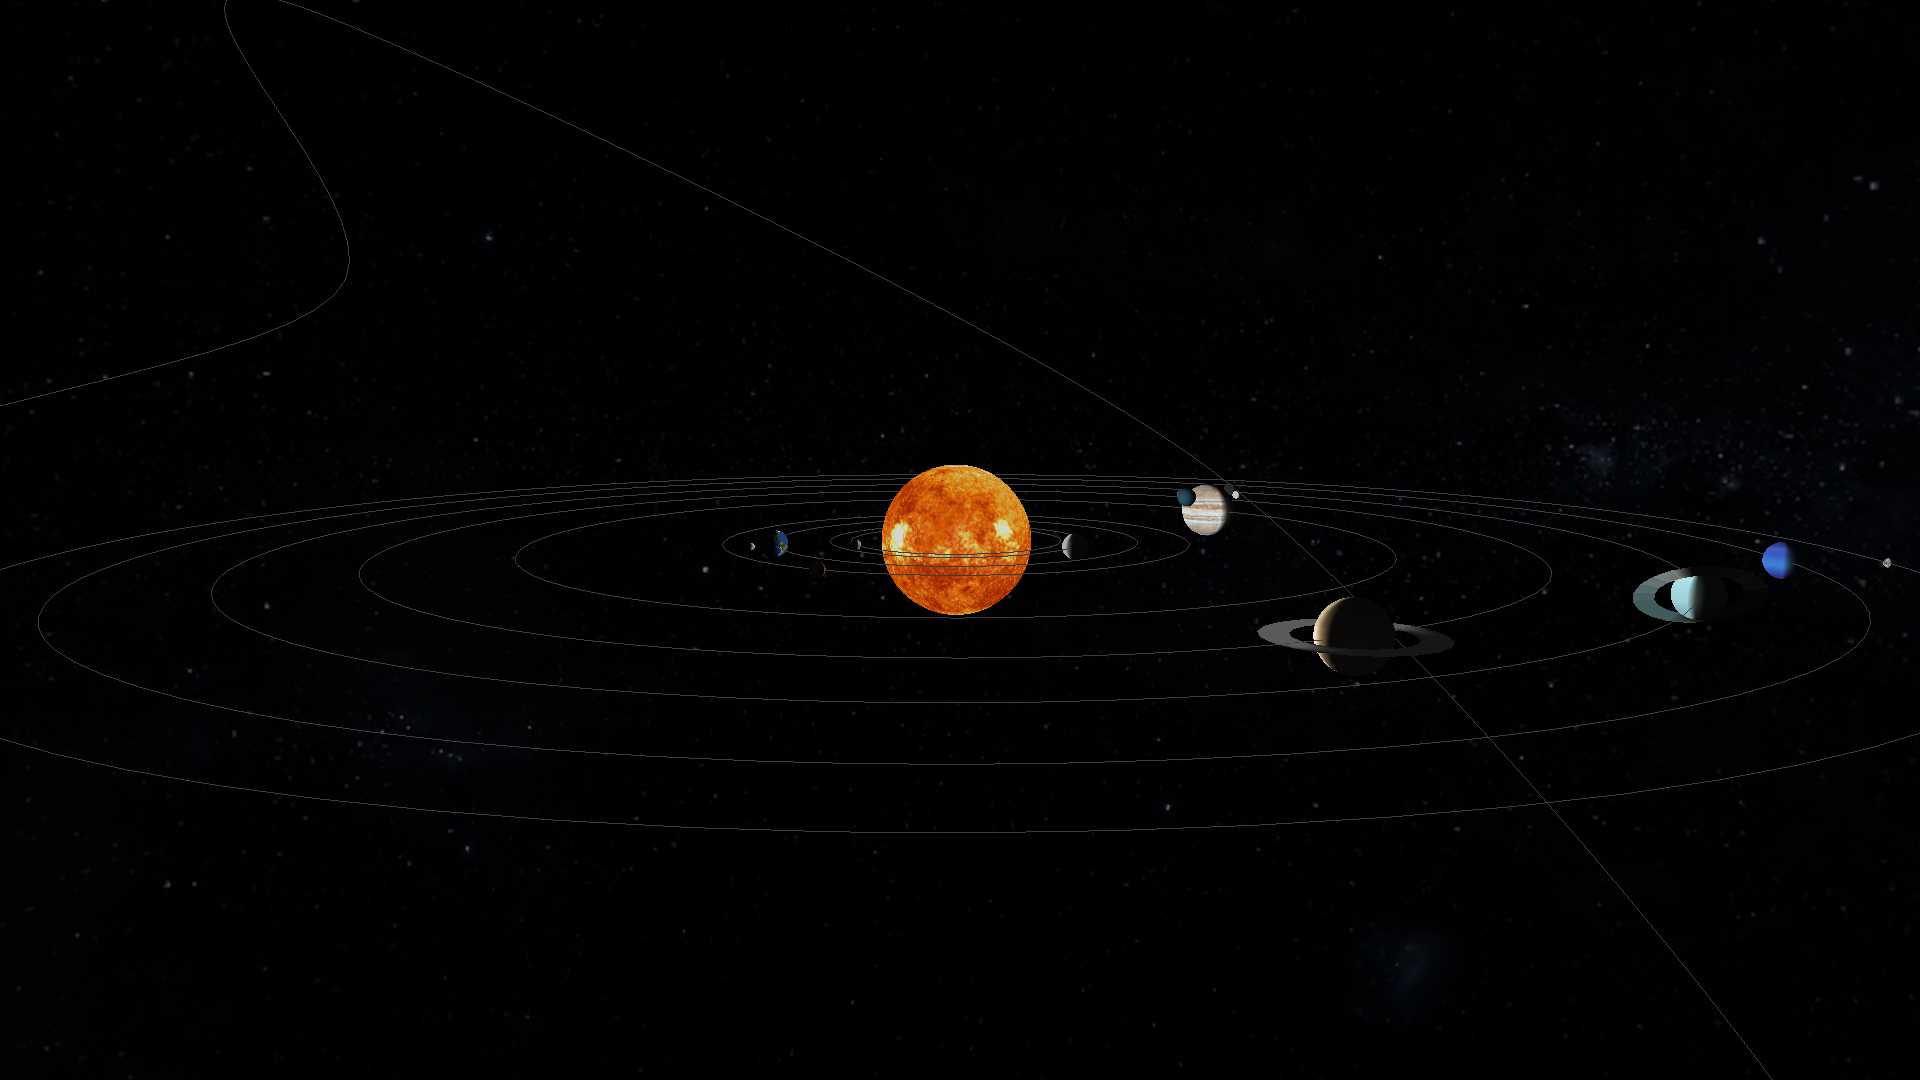
\includegraphics[width=\textwidth]{img/ex1.png}
    \caption{Renderização do modelo dinâmico do Sistema Solar}
\end{figure}

\begin{figure}[H]
    \centering
    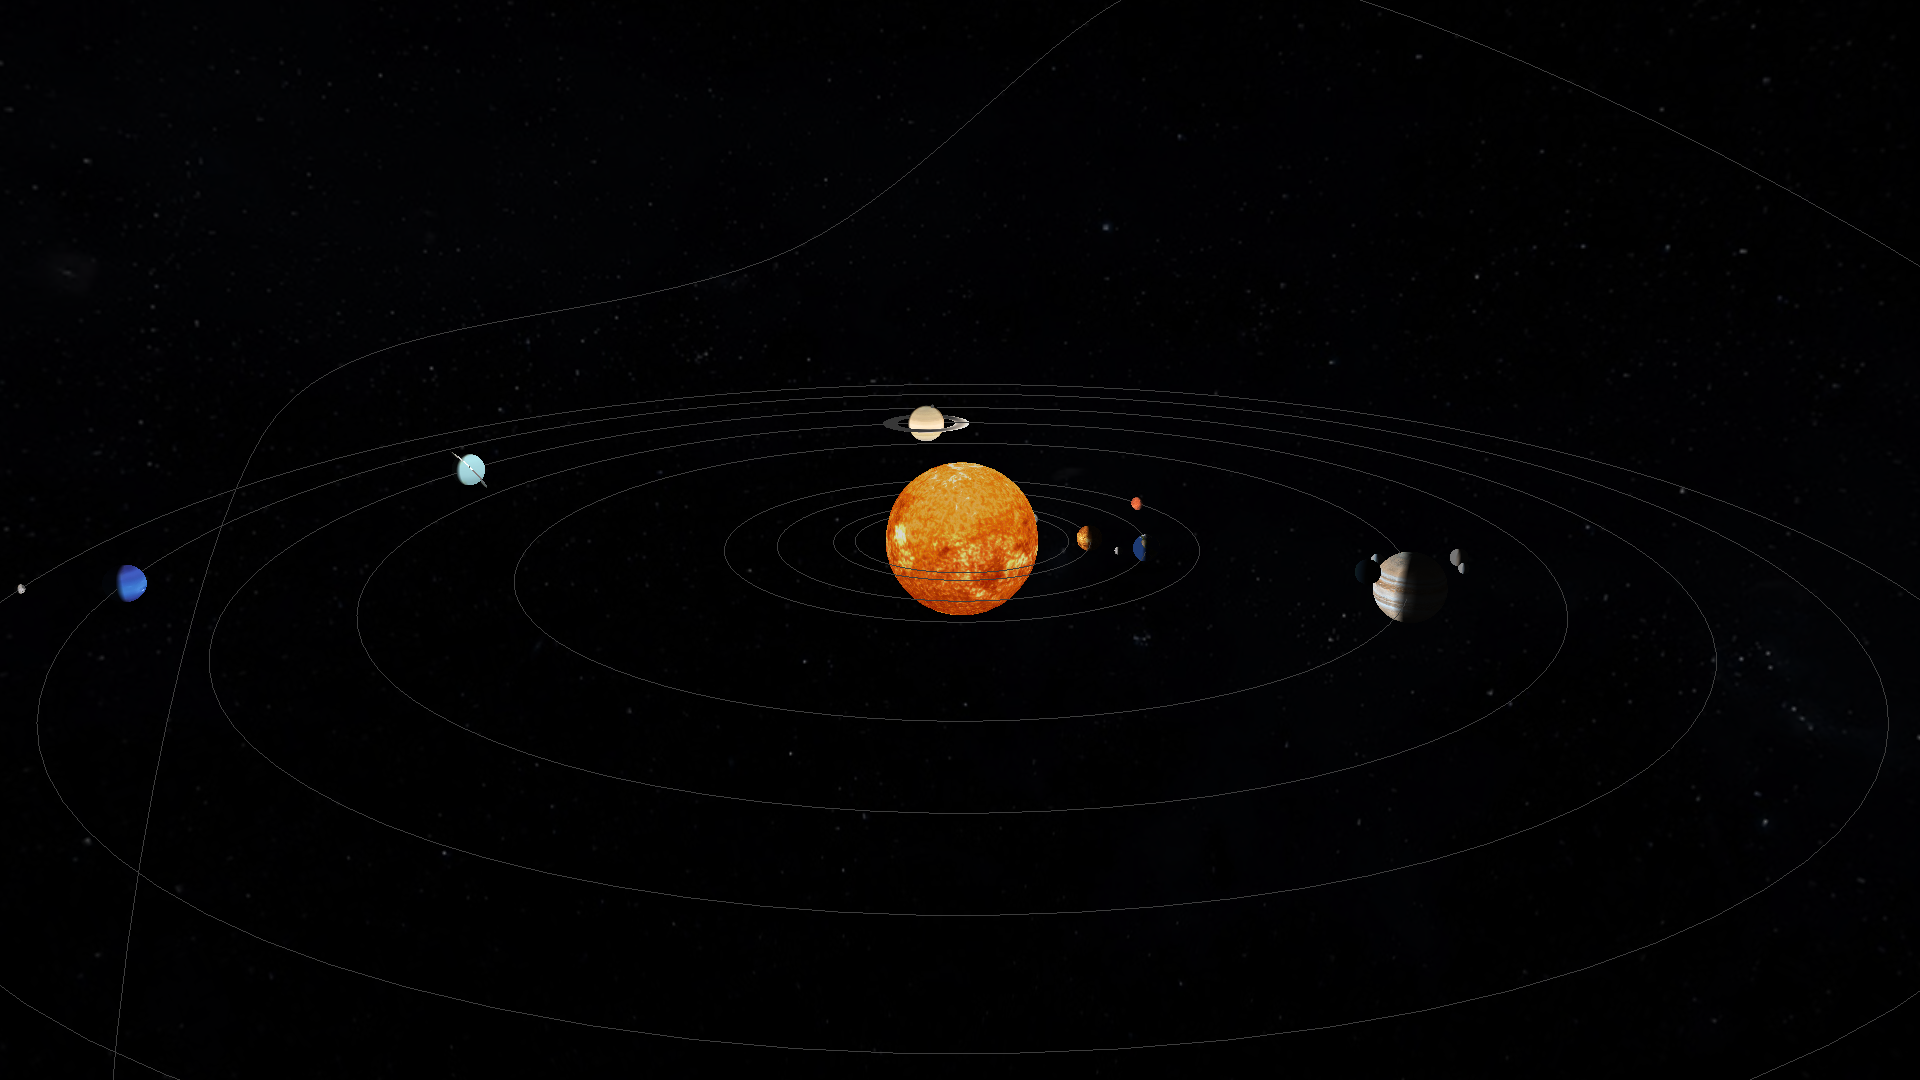
\includegraphics[width=\textwidth]{img/ex3.png}
    \caption{Renderização do modelo dinâmico do Sistema Solar}
\end{figure}

\begin{figure}[H]
    \centering
    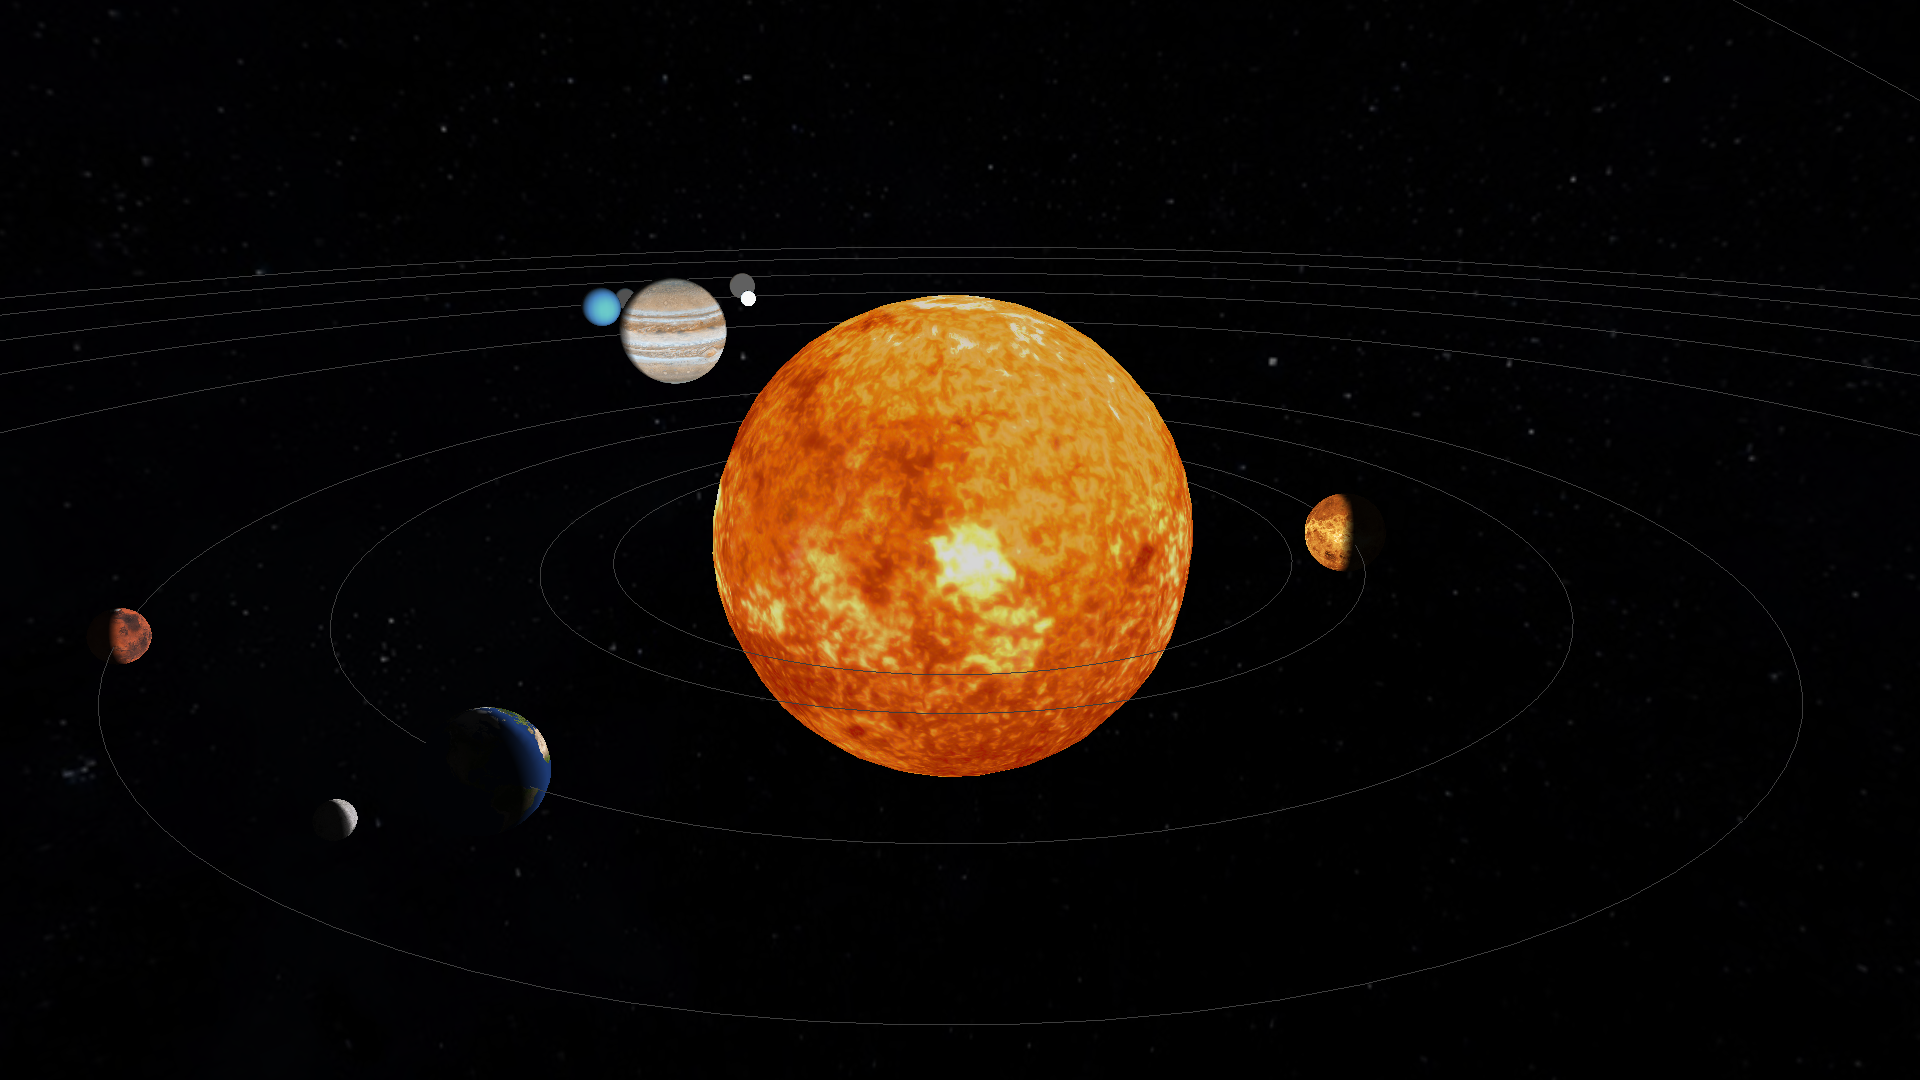
\includegraphics[width=\textwidth]{img/ex2.png}
    \caption{Renderização do modelo dinâmico do Sistema Solar}
\end{figure}

\pagebreak

\section{Conclusão}
A realização desta quarta e última fase do trabalho prático permitiu assimilar conhecimento 
relativo aos processos de iluminação e aplicação de texturas em Computação Gráfica. 

No entanto, o grupo deparou-se com algumas dificuldades, especialmente no que diz respeito ao 
mapeamento de uma textura a uma determinada figura. Tal deveu-se sobretudo ao facto de este 
mapeamento poder ser feito de várias formas. Apesar disto, após algumas tentativas e erros o 
grupo conseguiu superar o obstáculo com sucesso.

Em termos gerais, considera-se que o trabalho prático foi concluído com sucesso, permitindo 
desenvolver conhecimentos que relacionam a geometria à programação, assim como retratar 
cenários animados e com iluminação. Além disso, importa salientar que o trabalho desenvolvido 
permite gerar qualquer tipo de cenário através de um ficheiro XML, desde que este siga uma certa 
gramática.

\end{document}
